\documentclass[letterpaper,10pt]{article}

\usepackage[empty]{fullpage}
\usepackage{titlesec}
\usepackage[usenames,dvipsnames]{xcolor}
\usepackage{enumitem}
\usepackage[hidelinks]{hyperref}
\usepackage{fancyhdr}
\usepackage[english]{babel}
\usepackage{graphicx}
\usepackage{multicol}
\usepackage{paracol}
\ifdefined\pdfglyphtounicode
  \input{glyphtounicode}
\fi

\pagestyle{fancy}
\fancyhf{}
\fancyfoot{}
\renewcommand{\headrulewidth}{0pt}
\renewcommand{\footrulewidth}{0pt}

\addtolength{\oddsidemargin}{-0.55in}
\addtolength{\evensidemargin}{-0.55in}
\addtolength{\textwidth}{1.1in}
\addtolength{\topmargin}{-.55in}
\addtolength{\textheight}{1.1in}

\urlstyle{same}
\raggedbottom
\raggedright
\setlength{\tabcolsep}{0in}
\setlength{\parskip}{0pt}
\setlength{\columnsep}{14pt}

\titleformat{\section}{
  \vspace{0pt}\scshape\raggedright\normalsize
}{}{0em}{}[\color{black}\titlerule\vspace{2pt}]
\titlespacing*{\section}{0pt}{5pt}{2pt}

\ifdefined\pdfgentounicode
  \pdfgentounicode=1
\fi

% Tight bullet
\newcommand{\rItem}[1]{\item\footnotesize{#1\vspace{-1pt}}}

% One-line entry: role | company ............. date
\newcommand{\entry}[2]{%
  \vspace{1pt}
  \begin{tabular*}{\linewidth}{@{}l@{\extracolsep{\fill}}r@{}}
    \small\textbf{#1} & \footnotesize #2
  \end{tabular*}\vspace{-4pt}
}

% Project entry: name [tech] ............. year
\newcommand{\proj}[3]{%
  \vspace{2pt}
  \begin{tabular*}{\linewidth}{@{}l@{\extracolsep{\fill}}r@{}}
    \small\textbf{#1}\hspace{4pt}{\scriptsize\textit{#2}} & \footnotesize #3
  \end{tabular*}\vspace{-4pt}
}

\newcommand{\iStart}{\begin{itemize}[topsep=1pt,itemsep=0pt,parsep=0pt,leftmargin=10pt]}
\newcommand{\iEnd}{\end{itemize}\vspace{1pt}}

\begin{document}

% ═══════════════════════════════════════════════════════
%  HEADING: photo left, name + contacts right
% ═══════════════════════════════════════════════════════
\begin{minipage}[t]{0.16\textwidth}
  \vspace{0pt}
  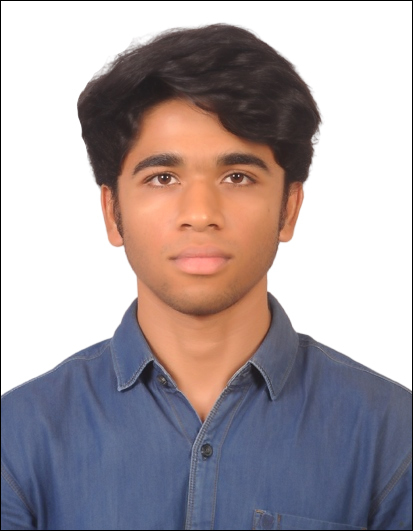
\includegraphics[width=\linewidth]{picture2.jpg}
\end{minipage}%
\hspace{6pt}%
\begin{minipage}[t]{0.82\textwidth}
  \vspace{16pt}
  {\LARGE\scshape\textbf{Aniruddh Ballal}}\\[2pt]
  \footnotesize
  +91-9731006863 \;$\cdot$\;
  \href{mailto:aniruddhballaldeeksha@gmail.com}{aniruddhballaldeeksha@gmail.com} \;$\cdot$\;
  \href{https://aniruddhballalportfolio.vercel.app}{aniruddhballalportfolio.vercel.app}\\[1pt]
  \href{https://linkedin.com/in/aniruddh-ballal-979797276}{linkedin.com/in/aniruddh-ballal-979797276} \;$\cdot$\;
  \href{https://github.com/aniruddhballal}{github.com/aniruddhballal} \;$\cdot$\;
  Bengaluru, KA\\[10pt]

  {\small Engineer working across physics and production software, from solar coronal-field simulations and orbital mechanics to full-stack financial systems and modelling. Strong in end-to-end development, scientific simulation, and debugging complex systems, with a focus on understanding how they behave.}
\end{minipage}

\vspace{4pt}
\noindent\rule{\textwidth}{0.4pt}

% ═══════════════════════════════════════════════════════
%  TWO-COLUMN BODY
%  Left (38%): Education · Skills · Community
%  Right (62%): Experience · Projects
% ═══════════════════════════════════════════════════════
\setlength{\columnseprule}{0.2pt}
\colseprulecolor{black!15}
\begin{paracol}{2}
\setcolumnwidth{0.36\textwidth, 0.60\textwidth}

% ─────────────────── LEFT COLUMN ───────────────────────
\section{Education}

\entry{Manipal Institute of Technology}{Manipal, KA}\\[6pt]
{\small\textit{B.Tech, Information Technology} \hfill \textit{Expected Jul 2026}}\\[2pt]
{\small CGPA: 8.1}

\vspace{8pt}

\entry{Deeksha Integrated PU College}{Yelahanka, KA}\\[4pt]
{\small Karnataka 2nd PUC (94.2\%)\hfill 2022}

\vspace{6pt}

\entry{Daffodils English School}{Sanjaynagar, KA}\\[4pt]
{\small ICSE 10th (92.9\%)\hfill 2020}\\[-2pt]
\section{Skills}

{\small\textbf{Languages}}\\[2pt]
{\small TypeScript, Python, JavaScript, Rust, Kotlin, C/C++, SQL}

\vspace{3pt}

{\small\textbf{Frontend \& Mobile}}\\[2pt]
{\small React, Next.js, React Native, Three.js, Tailwind CSS, MUI, Redux Toolkit}

\vspace{3pt}

{\small\textbf{Backend \& Data}}\\[2pt]
{\small FastAPI, Node.js, Express, PostgreSQL, SQLAlchemy, MongoDB, Firebase}

\vspace{3pt}

{\small\textbf{Scientific \& Systems}}\\[2pt]
{\small NumPy, SciPy, XGBoost, PuLP, Astropy, Matplotlib, WASM, Web Workers, GLSL, Git, Docker, KiCad}

\section{Experience}

\entry{Assistant Software Engineer $|$ Indiassetz}{Mar 2026--Oct 2026}\\[4pt]
{\small Modernised React Native applications and extended an existing CRM with payment reviews, approvals and revenue reporting. Developed a full-stack investor/back-office platform covering document governance, capital-call settlement tracking and portfolio reporting.}

\vspace{4pt}

\entry{Data Analyst Intern $|$ Qwixpert Consulting}{Jan--Mar 2026}\\[4pt]
{\small Analysed client data, automated reporting across Excel workbooks and prepared consulting presentations. Independently built decision-support tools for supply-chain network design, demand forecasting and dispatch planning.}

\vspace{4pt}

\entry{Frontend Web Dev Intern $|$ Indiassetz}{Jun--Jul 2025}\\[4pt]
{\small Collaborated with design and engineering teams to enhance UI/UX with React and Material UI; implemented micro-interactions and component redesigns using clean, reusable, version-controlled code.}

\vspace{4pt}

\entry{Solar Physics Intern $|$ Dept. of Physics, IISc}{Jun--Aug 2024}\\[4pt]
{\small Worked under Dr. Prantika Bhowmik on a Python project modelling and visualising solar magnetic-field evolution and cycles with spherical harmonics, SciPy, AstroPy, NumPy, and Matplotlib; derived quantitative insights into solar-cycle behaviour.}

\vspace{4pt}

% ─────────────────── RIGHT COLUMN ──────────────────────
\switchcolumn

\section{Community}

\entry{Astronomy Club, MIT Manipal}{Feb 2024 -- Apr 2025}\\[4pt]
{\small Managing Committee Member; completed coursework in AstroTech, black holes, astrobiology, and data-driven astronomy; organised club events and outreach.}

\vspace{6pt}

\entry{Revels PnP, MIT Manipal}{Jan -- Mar 2024}\\[4pt]
{\small Led a 4-person team to paint 10+ large acrylic posters and build 3D models for MIT’s annual cultural festival (25,000+ attendees).}

\vspace{6pt}

\entry{Manipal Runners' Club}{Dec 2023 -- Feb 2024}\\[4pt]
{\small Co-organised the Manipal Marathon 2024 (8,000+ participants) and coached enrollees through a 6-week training programme.}

\vspace{6pt}

\entry{Junior Avionics Member $|$ ThrustMIT}{Nov 2022--Nov 2023}\\[4pt]
{\small Built avionics for student rocketry: custom PCBs, telemetry, RF/GPS/IMU integration, microcontrollers, and control theory.}

\section{Projects {\normalfont\scriptsize\textit{demos \& source: \href{https://aniruddhballalportfolio.vercel.app}{aniruddhballalportfolio.vercel.app}}}}

\proj{Sunalyse}{}{2025--26}\\[4pt]
{\small Mapped the Sun’s invisible coronal magnetic field into an explorable 3D scene across 181 Carrington Rotations; reconstructed curved field lines from magnetograms and cut processing time \textbf{7.6x}.}

\vspace{4pt}

\proj{Queen's Gambit 2.0}{}{2025--26}\\[4pt]
{\small Turned chess games into a file carrier: built a reversible system that hides arbitrary files in legal moves, protects them with authenticated encryption, and makes encryption/decryption \textbf{\textasciitilde38x/\textasciitilde37x faster}.}

\vspace{4pt}

\proj{Credex}{}{2026}\\[4pt]
{\small Built a digital trade desk for SMEs, connecting negotiation, payment, lending, and underwriting in one workflow; backed it with immutable records, cash-flow planning, and 300--900 credit scoring.}

\vspace{4pt}

\proj{LOANlo}{}{2025}\\[4pt]
{\small Turned loan applications into a complete review workflow, from guided onboarding and document submission to underwriter decisions and administrator-led recovery, with automated risk checks and layered access controls.}

\vspace{4pt}

\proj{VenPay}{}{2025}\\[4pt]
{\small Turned vendor credit into a trackable procurement workflow: companies request products, vendors approve them, and payments remain visible through flexible deadlines, partial settlement, and post-payment ratings.}

\vspace{4pt}

\proj{SatLies}{}{2026}\\[4pt]
{\small Made orbital mechanics explorable: users shape an orbit and watch Earth’s oblateness and lunar/solar gravity pull it away from a clean baseline in real time.}

\end{paracol}

\end{document}
